% !TeX spellcheck = it_IT
\newpage
\section{Modello relazionale}
Il modello relazionale fu presentato da E. F. Codd nel 1970 per favorire l'\textbf{indipendenza} dei dati. Si basa sul concetto di \textbf{relazione}, la quale ha come rappresentazione la \textbf{tabella}.\\
In ogni base di dati distinguiamo lo \textbf{schema relazionale}, invariato nel tempo e che descrive la struttura) e l'\textbf{istanza}, ovvero i valori attuali.

\subsection{Matematica}
In matematica definiamo una \textbf{relazione} come l'insieme dei \textbf{domini}
\begin{equation*}
	D_1, \ldots, D_n
\end{equation*}
Inoltre il \textbf{prodotto cartesiano} $D_1 \times \ldots \times D_n$è l'insieme di tutte le \textbf{n-uple} $(d_1, \ldots, d_n)$ tali che 
\begin{equation*}
	d_1 \in D_1, \ldots, d_n \in D_n
\end{equation*}

\begin{example}[Relazioni in matematica]
	Dati i domini
	\begin{equation*}
		D_1 = \{a,b\} \qquad D_2 = \{x,y,z\}
	\end{equation*}
	il prodotto cartesiano è
	\begin{equation*}
		D_1 \times D_2 = \{(a, x), (a, y), (a, z), (b, x), (b,y), (b,z)\}
	\end{equation*}
	mentre una relazione possibile è
	\begin{equation*}
		r \subseteq D_1 \times D_2 = \{(a,x),(a,z), (b,y)\}
	\end{equation*}
\end{example}

\subsection{Modello}
I meccanismi per definire una BD con il modello relazionale sono la \textbf{ennupla} (insieme finito di coppie (Attributo, Tipo elementare)) e la \textbf{relazione}.

\begin{definition}[Schema di relazione]
	Uno schema di relazione $R(T)$ è una coppia formata da un \textbf{nome} $R$ e da un \textbf{tipo} $T$ definito come segue:
	\begin{itemize}
		\item \textit{int}, \textit{real}, \textit{boolean} e \textit{string} sono tipi \textbf{primitivi}
		\item $T=(A_1:T_1, \ldots, A_n:T_n)$ è un tipo \textbf{ennupla} di \textbf{grado} $n$ se $T_1, \ldots, T_n$ sono tutti tipi primitivi e se $A_1, \ldots, A_n$ sono etichette distinte dette \textbf{attributi}
		\item Due ennuple sono uguali se hanno uguale il grado, gli attributi e il tipo degli attributi con lo stesso nome
		\item L'ordine degli attributi non importa
		\item Se $T$ è tipo ennupla allora $\{T\}$ è un insieme di ennuple o tipo \textbf{relazione}
		\item Due tipi relazione sono uguali se hanno lo stesso tipo ennupla
	\end{itemize}
\end{definition}

\begin{definition}[Schema relazionale]
	Uno schema relazionale è costituito da schemi di relazione $R_i:\{T_i\} \quad i=1, \ldots, k$ e da un insieme di relativi \textbf{vincoli di integrità}.
\end{definition}

\begin{definition}[Ennupla]
	Un'ennupla $t = (A_1:V_1, \ldots, A_n:V_n)$ di tipo $T=(A_1:T_1, \ldots, A_n:T_n)$ è un insieme di coppie $(A_i, V_i)$ con $V_i$ di tipo $T_i$. Due ennuple sono uguali se hanno lo stesso insieme di coppie.
\end{definition}

\begin{definition}[Istanza]
	Un’istanza dello schema $R_i : \{T_i\}$ o \textbf{relazione} è un insieme finito di ennuple $\{t_1, t_2 , \ldots, t_k\}$, con ti di tipo $T_i$. La sua \textbf{cardinalità} è il numero delle sue ennuple. L'istanza di uno schema relazionale è formata da un'istanza di ogni suo schema di relazione.
\end{definition}

\subsubsection{Tabella}
Una tabella rappresenta una \textbf{relazione} se:
\begin{itemize}
	\item I valori di ogni colonna sono fra loro omogenei
	\item Le righe sono diverse fra loro
	\item Le intestazioni delle colonne sono diverse tra loro
\end{itemize}
L'ordinamento di righe e colonne non è importante.

\begin{center}
	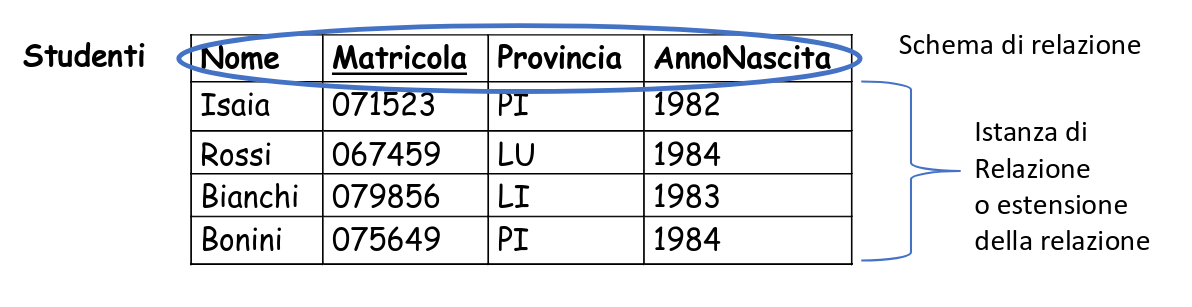
\includegraphics[scale=0.35]{schemarel.png}
\end{center}

\subsection{Valori}
Il modello relazionale è basato su \textbf{valori}, ovvero i riferimenti fra i dati in relazioni diverse sono rappresentati per mezzo di valori dei domini che compaiono nelle ennuple. Questo permette di mantenere \textbf{indipendenza} dalle strutture fisiche, si rappresenta solo i dati necessari e si garantisce \textbf{portabilità}.

\begin{definition}[Valore nullo]
	Il valore nullo denota l'assenza di un valore del dominio.
\end{definition}

\begin{definition}[Valore]
	$t[A]$, per ogni attributo $A$, è un valore nel dominio $dom(A)$ oppure il valore nullo $NULL$.
\end{definition}

\subsection{Vincoli di integrità}
Uno schema relazionale è costituito da un insieme di \textbf{schemi di relazione} e da un insieme di \textbf{vincoli d'integrità} su i possibili valori delle estensioni delle relazioni. Questi ultimi permettono di descrivere più accuratamente la realtà migliorando la \textbf{qualità dei dati} e aiutando nella progettazione

\begin{definition}[Vincolo d'integrità]
	Un vincolo d’integrità è una proprietà che deve essere soddisfatta dalle istanze che rappresentano informazioni corrette per l’applicazione. È espresso mediante una funzione booleana che associa ad ogni istanza il valore vero o falso.
\end{definition}

Esistono due tipi di vincoli: 
\begin{itemize}
	\item \textbf{Intrarelazionali}: devono essere rispettati dai valori contenuti nella relazione considerata. Possono essere sui valori o sulle ennuple.
	\item \textbf{Interrelazionali}: devono essere rispettati da valori contenuti in relazioni diverse
\end{itemize}

\subsubsection{Vincoli di ennupla}
Questi vincoli esprimono condizioni sui valori di ciascuna ennupla, indipendentemente dalle altre. Quando coinvolgono un solo attributo sono chiamati \textbf{vincoli di dominio}.

\newpage
\subsection{Chiave}
Una chiave è un insieme di attributi che identificano le ennuple di una relazione.
\begin{definition}[Chiave]
	Un insieme $K$ di attributi per uno schema di relazione $r$ è:
	\begin{itemize}
		\item \textbf{Superchiave} se $r$ non contiene due ennuple distinte $t_1$ e $t_2$ con $t_1[K]=t_2[K]$
		\item \textbf{Chiave} se è una superchiave \textbf{minimale}, cioè se non contiene un'altra superchiave
	\end{itemize}
\end{definition}
\begin{definition}[Chiave primaria]
	La chiave primaria di uno schema di relazione è una delle chiavi, di solito quella con il minor numero di attributi. Non ammette valori nulli ed è indicata con la sottolineatura.
\end{definition}

\begin{center}
	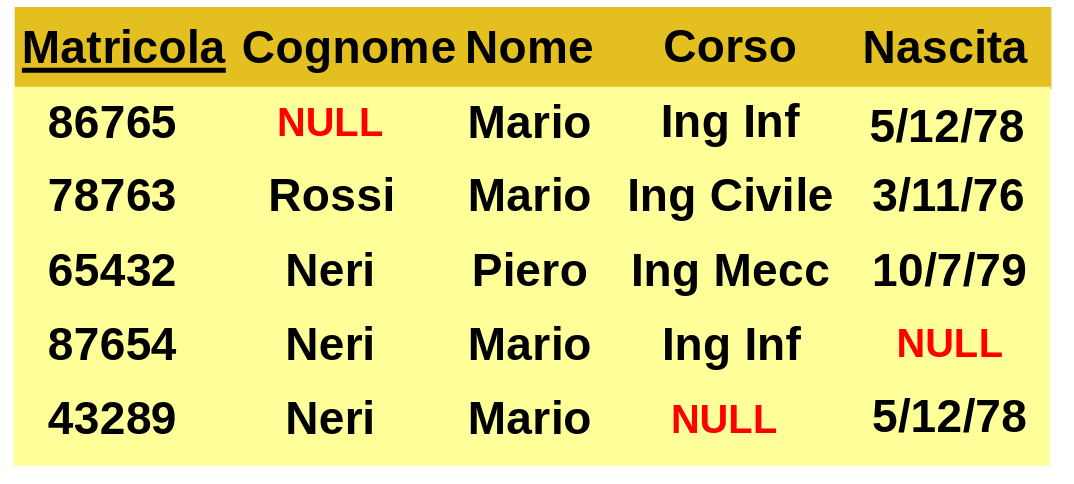
\includegraphics[scale=0.2]{chiave.png}
\end{center}

\begin{note}
	È possibile che esistano degli insiemi di attributi che soddisfino casualmente tutti i vincoli per essere chiavi, ma questo deve succedere \textbf{sempre} per tutte le istanze.
\end{note}

\begin{observation}[Esistenza]
	Ogni relazione ha come superchiave l'insieme di tutti gli attributi su cui è definita, quindi ha sempre almeno una chiave.
\end{observation}

\subsection{Integrità referenziale}
Nel modello relazionale le informazioni in relazioni sono correlate attraverso \textbf{valori} comuni, spesso quelli delle \textbf{chiavi primarie}. Deve quindi esserci una \textbf{coerenza}.\\
Gli attributi che permettono le correlazioni sono indicati sia con la sottolineatura (\textbf{chiavi esterne}) che con l'asterisco.
\begin{center}
	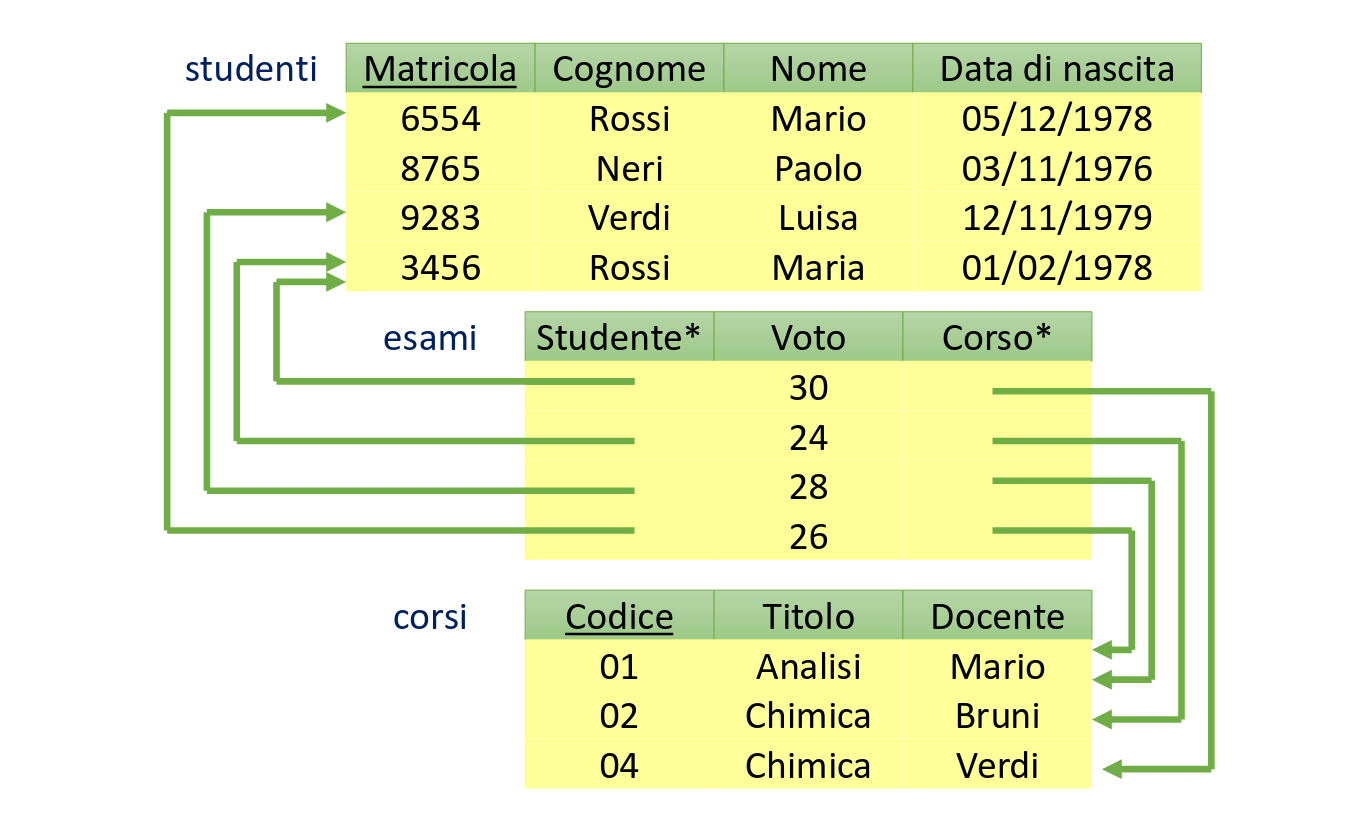
\includegraphics[scale=0.3]{chiaviesterne.png}
\end{center}

\subsubsection{Integrità referenziale}
\begin{definition}[Vincolo di integrità referenziale]
	Un vincolo di integrità referenziale (\textbf{foreign key}) fra gli attributi $X$ di una relazione $R_1$ e un’altra relazione $R_2$ impone ai valori su $X$ in $R_1$ di comparire come valori della chiave primaria di $R_2$.
\end{definition}
In caso di violazione del vincolo di integrità (e.g. viene eliminata una ennupla dalla tabella riferita), è possibile:
\begin{itemize}
	\item Rifiutare l'operazione
	\item Eliminare in cascata nelle altre tabelle
	\item Introdurre valori nulli
\end{itemize}

\begin{note}
	È possibile avere più chiavi esterne e in questo caso ci sono \textbf{vincoli multipli}.
\end{note}